\documentclass{article}
\usepackage[a4paper]{geometry}
\usepackage[brazil]{babel}
\usepackage[utf8]{inputenc}
\usepackage{url}
\usepackage{hyperref}
\usepackage{graphicx}
\usepackage{amsmath}
\usepackage{amsfonts}
\usepackage{amssymb}
\usepackage{pdfpages}

\usepackage{algorithm}
\usepackage[noend]{algpseudocode}
\algnewcommand\algorithmicforeach{\textbf{for each}}
\algdef{S}[FOR]{ForEach}[1]{\algorithmicforeach\ #1\ \algorithmicdo}

\title{Atividade 3 - Técnica de Relaxação Lagrangiana para o kSTSP}
\author{
	Lucas Guesser Targino da Silva - RA: 203534 \\
    Renan Fernando Franco da Silva - RA: 223989
}

\newcommand{\secref}[1]{(Seção \ref{#1})}
\newcommand{\subsecref}[1]{(Subseção \ref{#1})}
\newcommand{\constraintRef}[1]{Restrição \ref{#1}}
\newcommand{\figref}[1]{Figura \ref{#1}}

\newcommand{\Set}[1]{\ensuremath{\left\{#1\right\}}}
\newcommand{\partsof}[1]{\ensuremath{\mathcal{P}\left(#1\right)}}
\newcommand{\Sum}[1]{\ensuremath{\displaystyle\sum\limits_{#1}}}
\newcommand{\abs}[1]{\ensuremath{\left| #1 \right|}}
\newcommand{\binary}{\ensuremath{\Set{0, 1}}}

\newcommand{\edge}{\ensuremath{e}}
\newcommand{\edges}{\ensuremath{E}}
\newcommand{\vertex}{\ensuremath{v}}
\newcommand{\vertices}{\ensuremath{V}}
\newcommand{\nvertices}{\ensuremath{\abs{\vertices}}}
\newcommand{\ncycles}{2}
\newcommand{\allCycles}{\ensuremath{\Set{1, \ncycles}}}
\newcommand{\cycle}{\ensuremath{k}}
\newcommand{\subvertices}{\ensuremath{S}}
\newcommand{\graph}{\ensuremath{G}}
\newcommand{\cost}[1]{\ensuremath{c^{#1}}}
\newcommand{\costk}{\ensuremath{\cost{\cycle}}}
\newcommand{\costke}{\ensuremath{\cost{\cycle}_{\edge}}}
\newcommand{\Cost}{\ensuremath{\mathcal{C}}}
\newcommand{\Costke}{\ensuremath{\Cost^{\cycle}_{\edge}}}
\newcommand{\positiveReal}{\ensuremath{\mathbb{R}_+}}
\newcommand{\X}{\ensuremath{x}}
\newcommand{\xke}{\ensuremath{\X^{\cycle}_{\edge}}}
\newcommand{\Z}{\ensuremath{z}}
\newcommand{\ze}{\ensuremath{z_{\edge}}}
\newcommand{\similarity}{\ensuremath{\sigma}}
\newcommand{\totalconstraints}{\ensuremath{T_r}}
\newcommand{\bigo}[1]{\ensuremath{\mathcal{O}\left( #1 \right)}}

\newcommand{\lowerbound}{\ensuremath{z_{LB}}}
\newcommand{\upperbound}{\ensuremath{z_{UB}}}
\newcommand{\learningrate}{\ensuremath{\pi}}
\newcommand{\runningtime}{\ensuremath{\tau}}

\newcommand{\lagrange}{\ensuremath{\lambda}}
\newcommand{\lagrangeke}{\ensuremath{\lagrange_{\edge}^{\cycle}}}

\begin{document}

\maketitle

\section{Enunciado do Problema}

Sejam:

\begin{enumerate}
    \item $\graph = \langle \vertices,\edges \rangle$: um grafo não-orientado completo:
    \begin{enumerate}
        \item $\vertices$: conjunto de vértices;
        \item $\edges$: conjunto das arestas;
    \end{enumerate}
    \item $\costk: \edges \rightarrow \positiveReal,\ \forall \cycle \in \allCycles$, duas funções custo nos vértices;
        \begin{enumerate}
            \item dada uma aresta $\edge$, escrevemos $\costk(\edge) = \costke$;
        \end{enumerate}
    \item $\similarity$: parâmetro de similaridade de ciclos;
\end{enumerate}

Objetivo: encontrar dois ciclos Hamiltonianos com custo total mínimo, tal que pelo menos $\similarity$ arestas do grafo sejam visitadas por ambos os ciclos.

O nome kSTPS significa \textit{k-similar Travelling Salesman Problem}. O \textit{k} é o parâmetro de similaridade $\similarity$ acima, convenientemente renomeado para que não houvesse confusão com o $\cycle$ utilizado para indexar cada um dos ciclos (mais sobre isso na Seção \ref{sec:mathematical model}).

\section{Modelo Matemático}
\label{sec:mathematical model}

Nessa seção, será apresentada a formulação do problema utilizando Programação Linear Inteira. Esse não foi resolvido diretamente (já que não é o intuito da atividade), mas foi utilizado para derivar uma Relaxação Lagrangiana \secref{sec:lagrangian relaxation}, que foi modelo de fato implementado e resolvido.

\subsection{Variáveis de Decisão}
\label{constraint:variables}

\begin{itemize}
	\item $\xke$: presença da aresta $\edge$ no ciclo $\cycle$;
	\item $\ze$: presença de duplicação da aresta $\edge$;
\end{itemize}

Todas as variáveis de ``presença'' são decisões binárias com a seguinte interpretação de valores:

\begin{itemize}
	\item[0]: ausente
	\item[1]: presente
\end{itemize}

\subsection{Problema de Otimização}
\label{subsec:problem}

Minimizar:
\begin{equation}
    \label{eq:goal}
 	\Sum{\cycle \in \allCycles}
 	\Sum{\edge \in \edges}
 	\costke \ \xke
\end{equation}

Sujeito a:
\begin{equation}
	\label{constraint:vertex presence}
	\Sum{\edge \in \delta(\vertex)} \xke = 2
	\qquad
	\forall \vertex \in \vertices,
	\forall \cycle \in \allCycles
\end{equation}

\begin{equation}
	\label{constraint:no subcycle}
	\Sum{\edge \in \edges(\subvertices)} \xke \leqslant \abs{\subvertices} - 1
	\qquad
	\forall
		\subvertices \subsetneq \vertices,
		\subvertices \neq \emptyset,
		\forall \cycle \in \allCycles
\end{equation}

\begin{equation}
	\label{constraint:similarity compatibility}
	\xke \geqslant \ze
	\qquad
	\forall \edge \in \edges,
	\forall \cycle \in \allCycles
\end{equation}

\begin{equation}
	\label{constraint:similarity}
	\Sum{\edge \in \edges} \ze \geqslant \similarity
\end{equation}

\begin{equation}
	\label{constraint:binary variables}
	\xke, \ze \in \binary
	\qquad
	\forall \edge \in \edges,
	\forall \cycle \in \allCycles
\end{equation}

\subsection{Explicação das Restrições}
\label{subsec: constraints explanation}

\begin{itemize}
    \item A função objetivo \eqref{eq:goal} é soma do custo de todas as arestas selecionadas em todos os ciclos.
    \item A restrição \eqref{constraint:vertex presence} garante que a quantidade de arestas incidentes em todos os vértices seja 2. Essa condição faz com que todos os vértices tenham que ser visitados (duas arestas pois uma é a de ``entrada'' e a outra a de ``saída'').
    \item A restrição \eqref{constraint:no subcycle} garante que não existam subciclos nos ciclos. Nessa restrição, $\subvertices$ é um subconjunto próprio e não-vazio dos vértices do problema. A expressão $\edges(\subvertices)$ é o conjunto das arestas cujos ambos os vértices estão em $\subvertices$.
    \item A restrição \eqref{constraint:similarity compatibility} garante que, se uma aresta foi escolhida para ser duplicada, então essa aresta aparecerá nos dois ciclos.
    \item A restrição \eqref{constraint:similarity} garante que pelo menos $\similarity$ arestas serão escolhidas para serem duplicadas.
    \item A restrição \eqref{constraint:binary variables} garante que todas as variáveis são decisões binárias, ou seja, assumem apenas um de dois possíveis valores: 0 e 1.
\end{itemize}

\subsection{Tamanho das Restrições}
\label{subsec:constraints size}

\begin{itemize}
	\item Restrição \eqref{constraint:vertex presence}: uma para cada vértice e para cada ciclo. Total: $\ncycles \cdot \abs{\vertices}$;
	\item Restrição \eqref{constraint:no subcycle}: uma para $\subvertices \in \partsof{\vertices}, \subvertices \neq \vertices, \subvertices \neq \emptyset$ e para cada ciclo. Total: $\ncycles \cdot \left( 2^{\abs{\vertices}} - 2\right)$;
	\item Restrições \eqref{constraint:similarity compatibility}: uma para cada aresta e para cada ciclo. Total: $\ncycles \cdot \abs{\edges} = \ncycles \cdot \dfrac{\abs{\vertices}^2 - \abs{\vertices}}{2}$ (já que o grafo é completo);
	\item Restrições \ref{constraint:similarity}: apenas uma. Total: 1;
\end{itemize}

Assim, o número total de restrições é:

\begin{equation}
	\totalconstraints =
		  \ncycles \cdot \abs{\vertices}
		+ \ncycles \cdot \left( 2^{\abs{\vertices}} - 2\right)
		+ \ncycles \cdot \dfrac{\abs{\vertices}^2 - \abs{\vertices}}{2}
		+ 1
\end{equation}

Assim:

\begin{equation}
	\label{eq:number of constraints}
	\totalconstraints \in \bigo{2^{\nvertices}}
\end{equation}

Note que há um número exponencial de restrições.

% Na implementação computacional do problema, não é possível adicionar tantas restrições por falta de recursos computacionais (memória e processamento). Há entretanto uma forma de contornar o problema atŕavés do que se chama de \textit{lazy evaluation}. A ideia é não adicionar tais restrições no início. Conforme soluções factíveis são encontradas, verifica-se se há subciclos nelas e, caso sim, adiciona-se apenas as restrições necessárias para eliminar tais subciclos.
%
% Dependendo do caso em mãos, essa abordagem pode reduzir drasticamente o número de restrições e consequentemente acelerar a busca.

\section{Relaxação Lagrangiana}
\label{sec:lagrangian relaxation}

\subsection{Escolha da Restrição a ser Relaxada}

A técnica de Relaxação Lagrangiana consiste em escolher uma ou mais restrições para relaxar. Tal escolha visa remover as restrições que fazem do problem ``difícil de ser resolvido'' \cite{bib:linear-optimization-intro}.

\subsubsection{Análise das Restrições}

\begin{itemize}
	\item \constraintRef{constraint:vertex presence}: não parece ser uma restrição difícil;
	\item \constraintRef{constraint:no subcycle}: essa restrição é de fato difícil. Entretanto, há um número exponencial delas, de forma que é inviável relaxá-la. Além disso, há técnicas que lidam bem com ela\footnote{\textit{Lazy constraints} por exemplo, abordado no trabalho anterior.};
	\item \constraintRef{constraint:similarity compatibility}: no trabalho anterior, notou-se que o fator de similaridade causa bastante impacto no tempo computacional \figref{figure:previous running time}. Isso significa que ele deixa o problema difícil, sendo então um bom candidato à relaxação;
	\item \constraintRef{constraint:similarity}: essa restrição tem efeitos bem parecidos com a \constraintRef{constraint:similarity compatibility}. Ela representa, entretanto, apenas uma equação de restrição, não sendo assim interessante para a relaxação;
	\item \constraintRef{constraint:binary variables}: essa restrição faz parte do modelo relaxado;
\end{itemize}

Portanto, a restrição escolhida para ser relaxada é a \constraintRef{constraint:similarity compatibility}.

\begin{figure}[]
    \centering
    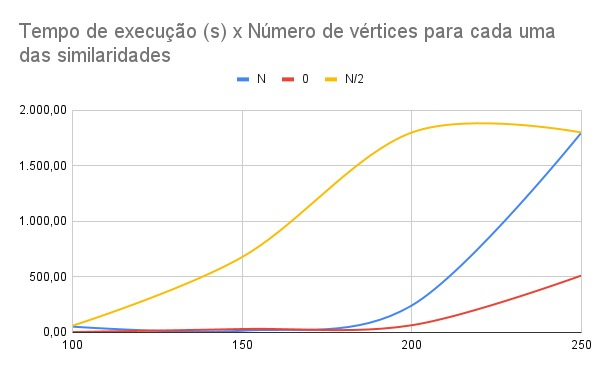
\includegraphics[width=0.7\textwidth]{images/running_time.jpeg}
    \caption{Tempo de execução dos experimentos do trabalho anterior.}
    \label{figure:previous running time}
\end{figure}

\subsection{Modelo Matemático da Relaxação Lagrangiana}
\label{subsec:lagrangian relaxation}

\begin{equation}
    \label{eq:goal lagrangian}
	\max_{\lagrange}
	\left\{
		\min_{\X, \Z}
 		\Sum{\cycle \in \allCycles}
 		\Sum{\edge \in \edges}
 		\Costke \ \xke
 		+ \lagrangeke \ze
 	\right\}
\end{equation}

Em que:

\begin{equation}
	\Costke = \costke - \lagrangeke
\end{equation}

Sujeito às restrições \ref{constraint:vertex presence}, \ref{constraint:no subcycle}, e \ref{constraint:similarity} do problema original \subsecref{subsec:problem}, e a restrições de domínio:

\begin{equation}
	\label{constraint:value of variables}
	0 \leqslant \xke, \ze \leqslant 1
	\qquad
	\forall \edge \in \edges,
	\forall \cycle \in \allCycles
\end{equation}

\begin{equation}
	\label{constraint: lagrange}
	\lagrangeke \geqslant 0
	\qquad
	\forall \edge \in \edges,
	\forall \cycle \in \allCycles
\end{equation}

Note que esse problema pode ser resolvido quebrando-o em $\ncycles$ TSP e um problema para resolver as arestas a serem duplicadas $\ze$. Tais detalhes são melhor descritos nas próximas subsubseções.

\subsubsection{Problema da escolha de ciclos derivado da Relaxação Lagrangiana}

Dado $\Cost$, minimizar:
\begin{equation}
 	\Sum{\cycle \in \allCycles}
 	\Sum{\edge \in \edges}
 	\Costke \ \xke
\end{equation}

Sujeito às restrições \ref{constraint:vertex presence}, \ref{constraint:no subcycle}, e \ref{constraint:binary variables}. Note que esse problema é o TSP.

\subsubsection{Problema da escolha das arestas similares derivado da Relaxação Lagrangiana}
\label{subsec:z problem}

Minimizar:
\begin{equation}
 	\Sum{\cycle \in \allCycles}
 	\Sum{\edge \in \edges}
	\lagrangeke \ze
\end{equation}

Sujeito à restrição \ref{constraint:binary variables} e:

\begin{equation}
	\Sum{\edge \in \edges} \ze \geqslant \similarity
\end{equation}

Esse problema é facilmente resolvido escolhendo-se entre as arestas $\edge \in \edges$, as $\similarity$ com menor peso $\Sum{\cycle \in \allCycles} \lagrangeke$. Para essas arestas, é dado o valor $1$ e para as outras é dado o valor $0$.

\subsection{Método do Subgradiente}
Vamos utilizar o Método do Subgradiente para resolver o dual lagrangiano mostrado na Secção 	\ref{constraint:binary variables}. No começo do método, inicializamos $\lambda$ e o \textit{learning rate} $\pi$, então temos um processo iterativo. Em cada iteração recebemos uma solução ótima para (9) usando o $\lambda$ atual, juntamente com o melhor \textit{upper bound} $z_{UB}$ e o \textit{lower bound} atual $z_{LB}^{(i)}$, e então atualizamos o $\lambda$ conforme o Algoritmo \ref{Subgradient}. Se de uma iteração para outra o \textit{lower bound} atual piorar, atualizamos o \textit{learning rate} fazendo $\pi = \pi \cdot \frac{\sqrt{5} - 1}{2}$.

\begin{algorithm}
\label{algorithm:subgradient}
\caption{Subgradient}
\label{Subgradient}
\begin{algorithmic}[1]
    \Function{Initialize}{$\lambda$, $\pi$}
        \State{$\lambda_e^k$ = $1$, para todo $\edge \in \edges$ e $k \in \{1, 2\}$}
        \State{$\pi \gets 2$}
        \State{\textbf{return} $\lambda, \pi$}
    \EndFunction
    \Function{Update}{$x$, $z$, $z_{UB}, z_{LB}^{(i)}$, $\lambda$, $\pi$}
        \State{$g_e^k = z_e - x_e^k$ para todo $\edge \in \edges$ e $k \in \{1, 2\}$}
        \State{$\alpha = \pi \frac{(z_{UB} - z_{LB})}{\sum_{k \in \{1, 2\}} \sum_{\edge \in \edges} (g_e^k)^2}$}
        \State{$\lambda_e^k = max(0, \lambda_e^k + \alpha \cdot g_e^k)$, para todo $\edge \in \edges$ e $k \in \{1, 2\}$}
        \State{\textbf{return} $\lambda$}
    \EndFunction
\end{algorithmic}
\end{algorithm}

\subsection{Heurística Lagrangiana}
Na Heurística Lagrangiana recebemos dois ciclos hamiltonianos $tour1$ e $tour2$, além de uma constante $\sigma$, então devemos retornar dois ciclos hamiltonianos $newTour1$ e $newTour2$ tais que os mesmos compartilham no mínimo $sigma$ arestas. Nosso algoritmo está a seguir:

\begin{algorithm}
\begin{algorithmic}[1]
\Function{Heuristic}{$tour1, tour2, \sigma$}
    \State{$equalEdges \gets$ arestas em comum entre $tour1$ e $tour2$}
    \State{$remainingEdges \gets$ arestas que não estão em ao menos um dos tours}
    \State{Ordene as arestas dos conjuntos $equalsEdges$ e $remainingEdges$ por seus custos, onde o custo de uma aresta é a soma dos valores do seu custo em cada tour}
    \State{$edges \gets$ concatenação de $equalsEdges$ e $remainingEdges$, nesta ordem}
    \State{$newTour1 \gets \emptyset$}
    \State{$newTour2 \gets \emptyset$}
    \State{$numSimilar \gets 0$}
    \For{cada aresta $e$ em $edges$}
        \If{$numSimilar \geq \sigma$}
            \State{\textbf{break}}
        \EndIf
        \If{$e$ não forma um subtour em $newTour1$ e $newTour2$}
            \State{$newTour1 \gets newTour1 \cup \{e\}$}
            \State{$newTour2 \gets newTour2 \cup \{e\}$}
            \State{$numSimilar \gets numSimilar + 1$}

        \EndIf
    \EndFor
    \State{$edgesTour1 \gets$ arestas do $tour1$ ordenadas por seu custo no $tour1$}
    \For{cada aresta $e$ em $edgesTour1$}
        \State{se $e$ não formar subtour em $newTour1$, adicione $e$ no mesmo}
    \EndFor

    \State{$edges1 \gets$ todas as arestas ordenadas por seu custo no $tour1$}
    \For{cada aresta $e$ em $edges1$}
        \State{se $e$ não formar subtour em $newTour1$, adicione $e$ no mesmo}
    \EndFor
    \\
    \State{$edgesTour2 \gets$ arestas do $tour2$ ordenadas por seu custo $tour2$}
    \For{cada aresta $e$ em $edgesTour2$}
        \State{se $e$ não formar subtour em $newTour2$, adicione $e$ no mesmo}
    \EndFor

    \State{$edges2 \gets$ todas as arestas ordenadas por seu custo no $tour2$}
    \For{cada aresta $e$ em $edges2$}
        \State{se $e$ não formar subtour em $newTour2$, adicione $e$ no mesmo}
    \EndFor
    \State{\textbf{return} $newTour1$ e $newTour2$}
\EndFunction
\end{algorithmic}
\end{algorithm}

\section{Algoritmo de Solução do Problema}

% how to write pseudocode in latex:
%   https://math-linux.com/latex-26/faq/latex-faq/article/how-to-write-algorithm-and-pseudocode-in-latex-usepackage-algorithm-usepackage-algorithmic
%  https://tex.stackexchange.com/questions/163768/write-pseudo-code-in-latex

\begin{algorithm}
\label{alg:kstsp}
\begin{algorithmic}
\Function{kSTSP}{$custos1, custos2, \similarity, \runningtime_{max}, \learningrate_{min}, \Delta_{min}$}
    \State{$\lagrange_0 \gets 1$}
    \State{$\runningtime \gets 0$}
    \State{$\learningrate \gets 2$}
    \State{$\Delta\lowerbound \gets +\infty$}
    \State{$\Delta\upperbound \gets +\infty$}
    \While{
        $\runningtime < \runningtime_{max}$
        or $\learningrate > \learningrate_{min}$
        or ($\Delta\lowerbound > \Delta_{min}$ and $\Delta\upperbound > \Delta_{min}$)
    }
    \State{$tsp1 \gets$ Solve-TSP($custos1$)}
    \State{$tsp2 \gets$ Solve-TSP($custos2$)}
    \State{$\Z \gets$ Resolve-z($\lagrange, \similarity$}
    \State{$ciclo1 \gets $ Heuristic($tsp1, tsp2, \similarity$)}
    \State{$ciclo2 \gets $ Heuristic($tsp2, tsp1, \similarity$)}
    \State{$\lowerbound, \Delta\lowerbound \gets $ Compute-Lower-Bound($ciclo1, ciclo2, \Z, \lagrange$)}
    \State{$\upperbound, \Delta\upperbound \gets $ Compute-Upper-Bound($ciclo1, ciclo2, \Z$)}
    \State{$\lagrange,  \gets$ Update($ciclo1, ciclo2, \Z,. \upperbound, \lagrange, \learningrate$)}
    \If{$\Delta\lowerbound < 0$}
        \State{$\learningrate \gets \dfrac{\sqrt{5} - 1}{2} \learningrate$}
    \EndIf
    \EndWhile
\EndFunction
\end{algorithmic}
\end{algorithm}

\section{Experimento Computacional}

\subsection{Configuração da Máquina}

O problema foi executado num ideapad S145 81S90005BR: Lenovo IdeaPad S145 Notebook Intel Core i5-8265U (6MB Cache, 1.6GHz, 8 cores), 8GB DDR4-SDRAM, 460 GB SSD, Intel UHD Graphics 620.

O sistema operacional foi o Fedora 35 executando gcc (GCC) 11.2.1 20220127 (Red Hat 11.2.1-9), Concorde \cite{bib:concorde} e o solver QSOpt \cite{bib:qsopt}.

Como linguagem de programação, utilizamos C++ \cite{bib:cpp}.

\subsection{Dados do Problema}

Os dados do problema foram fornecidos em um arquivo contendo 4 colunas e 250 linhas. A interpretação dos dados é a seguinte: cada linha representa um vértice e cada par de coluna as coordenadas desse vértice. A razão para um vértice ter duas posições diferentes é simplesmente para que as distâncias entre eles tenham valores diferentes no primeiro e no segundo ciclo.

O modelo na verdade precisa apenas de pesos. Construímos a primeira função de custo como a distância euclidiana entre os pontos das colunas 1 e 2. Da mesma forma, utilizamos distância euclidiana entre os pontos das colunas 3 e 4 para construir a segunda função de custo.

Note que, com essa interpretação, parece que temos dois conjuntos de vértices, um definido pelas colunas 1 e 2, e outro definido pelas colunas 3 e 4. Conforme explicitado no primeiro parágrafo da seção, esse não é o caso. Cada linha é um vértice e os valores fornecidos servem apenas para calcular a distância euclidiana e usá-la como peso para as arestas. Dessa forma, a aresta que liga os vértices representados pelas linhas 12 e 84, por exemplo, possui dois pesos diferentes, um para ser utilizado no primeiro ciclo e outro para ser utilizado no segundo.

\subsection{Geração das Instâncias}

Para gerar instâncias de um dado tamanho $N$, utilizamos as primeiras $N$ linhas dos dados fornecidos.

\section{Resultados dos Experimentos}

% \begin{table}[]
%     \centering
%     \begin{tabular}{|c|c|}
%         \hline
%         Variável & Descrição \\\hline
%         $\nvertices$ & Número de Vértices \\\hline
%         $\similarity$ & Fator de Similaridade \\\hline
%         $\upperbound$ & Limite superios (Upper Bound) \\\hline
%         $\lowerbound$ & Limite inferior (Lower Bound) \\\hline
%         $\learningrate$ & Learning Rate \\\hline
%     \end{tabular}
% \end{table}

\begin{table}[h]
    \label{tab:res}
    \centering
    \begin{tabular}{|c|c|c|c|c|c|}
        \hline
        \nvertices & \similarity & \upperbound & \lowerbound & opt gap & \runningtime \\\hline\hline
            100 & 0   & 1630 & 1627.41 & 0.002 & 609\\\hline
            100 & 100 & 3574 & 1842.37 & 0.940 & 329\\\hline
            100 & 50  & 2310 & 1720.67 & 0.343 & 240\\\hline
            150 & 0   & 1966 & 1961.29 & 0.002 & 605\\\hline
            150 & 150 & 4980 & 2331.49 & 1.136 & 618\\\hline
            150 & 75  & 3106 & 2137.31 & 0.453 & 507\\\hline
            200 & 0   & 2308 & 2292.01 & 0.007 & 619\\\hline
            200 & 100 & 3838 & 2516.89 & 0.525 & 617\\\hline
            200 & 200 & 6392 & 2766.68 & 1.310 & 635\\\hline
            250 & 0   & 2597 & 2571.7 & 0.010 & 733\\\hline
            250 & 125 & 4451 & 2833.34 & 0.571 & 700\\\hline
            250 & 250 & 7442 & 3076.08 & 1.419 & 616\\\hline
    \end{tabular}
    \caption{Resultados dos experimentos computacionais. \runningtime é o tempo de processamento em segundos.}
    \label{tab:results}
\end{table}

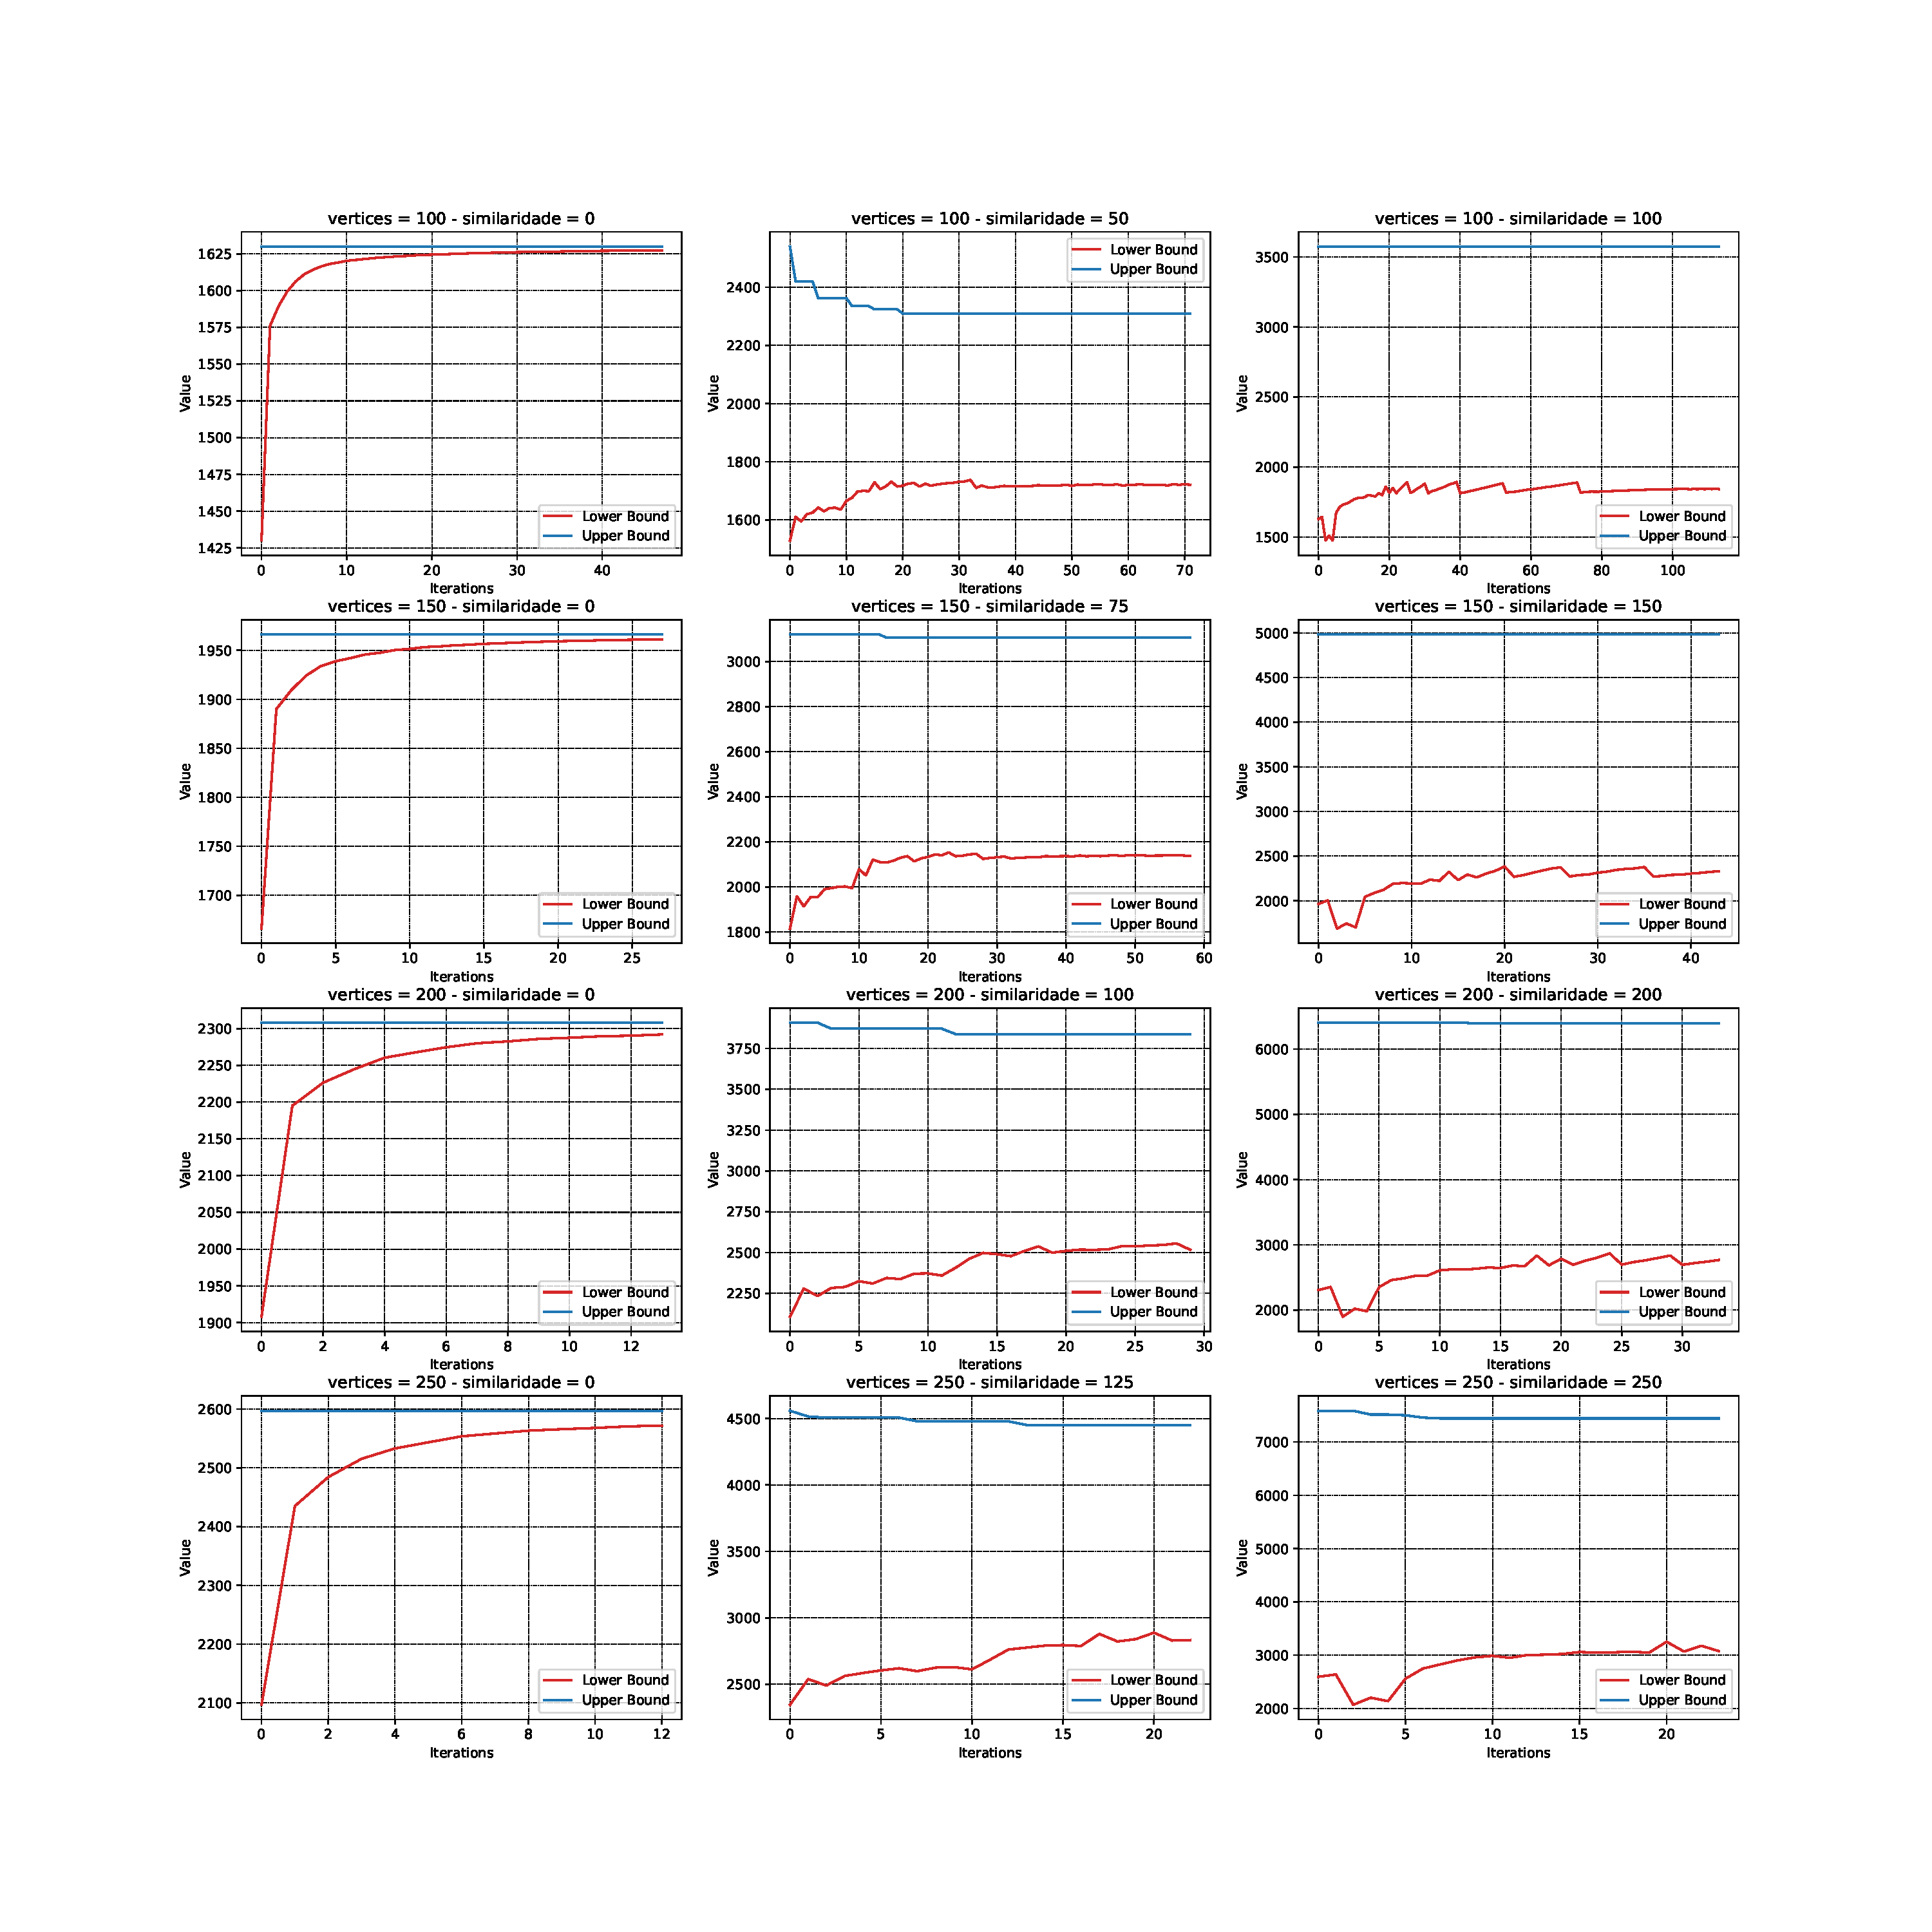
\includepdf{images/all.pdf}

% \begin{figure}[]
%     \centering
%     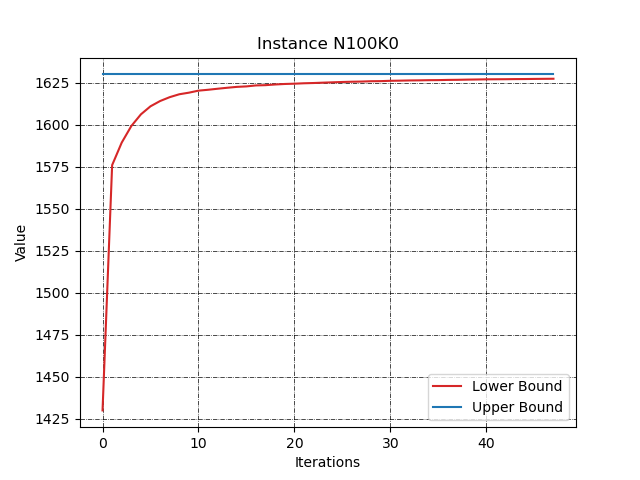
\includegraphics[width=\textwidth]{images/N100K0.png}
%     \label{fig:N100K0}
% \end{figure}

% \begin{figure}[]
%     \centering
%     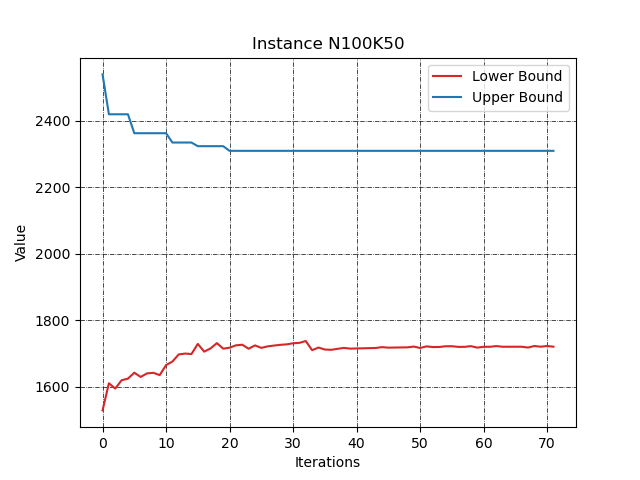
\includegraphics[width=\textwidth]{images/N100K50.png}
%     \label{fig:N100K50}
% \end{figure}

% \begin{figure}[]
%     \centering
%     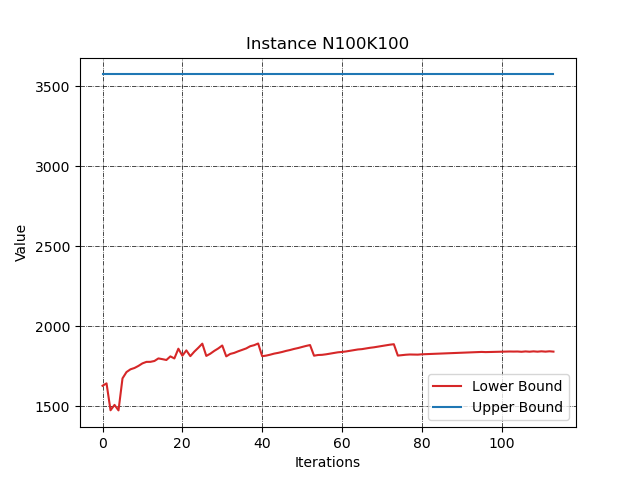
\includegraphics[width=\textwidth]{images/N100K100.png}
%     \label{fig:N100K100}
% \end{figure}

% \begin{figure}[]
%     \centering
%     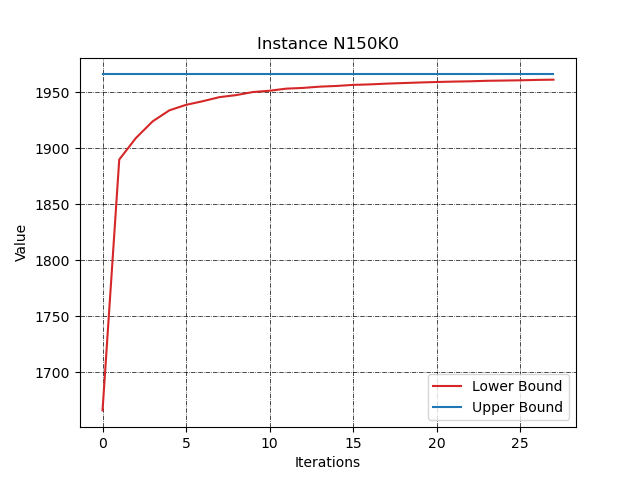
\includegraphics[width=\textwidth]{images/N150K0.png}
%     \label{fig:N150K0}
% \end{figure}

% \begin{figure}[]
%     \centering
%     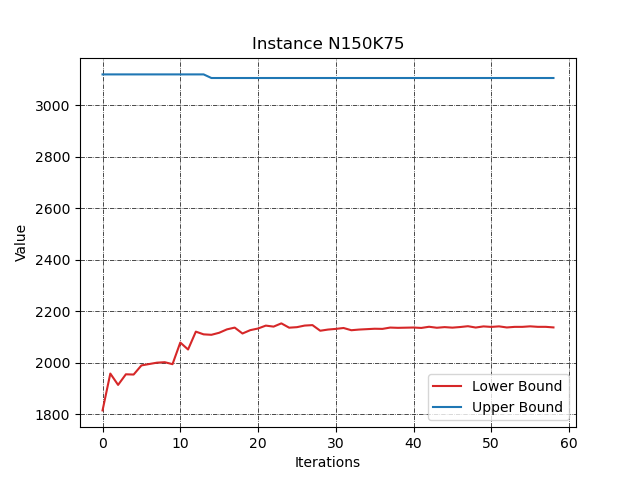
\includegraphics[width=\textwidth]{images/N150K75.png}
%     \label{fig:N150K75}
% \end{figure}

% \begin{figure}[]
%     \centering
%     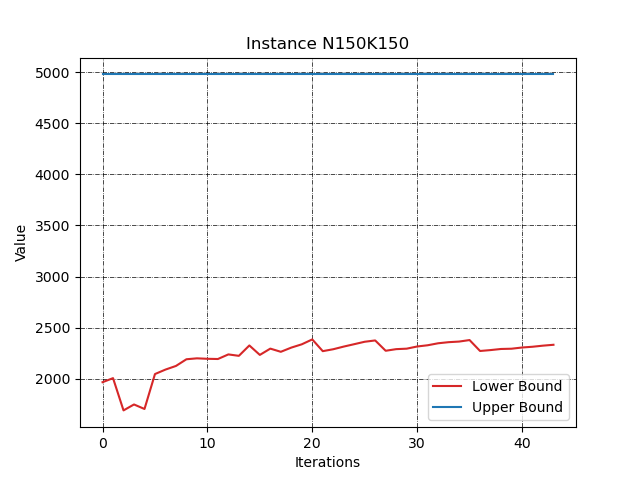
\includegraphics[width=\textwidth]{images/N150K150.png}
%     \label{fig:N150K150}
% \end{figure}

% \begin{figure}[]
%     \centering
%     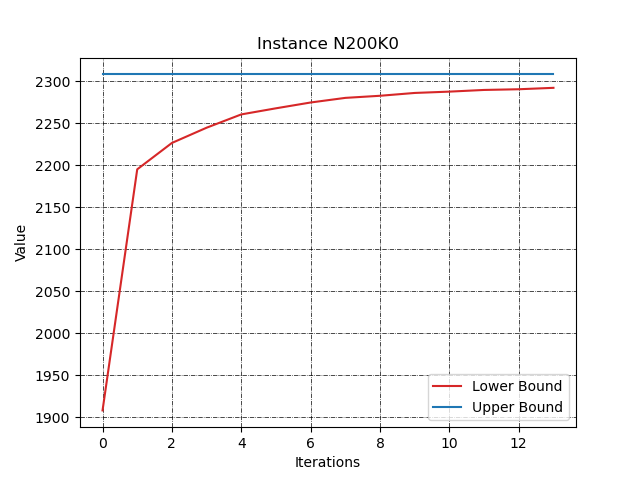
\includegraphics[width=\textwidth]{images/N200K0.png}
%     \label{fig:N200K0}
% \end{figure}

% \begin{figure}[]
%     \centering
%     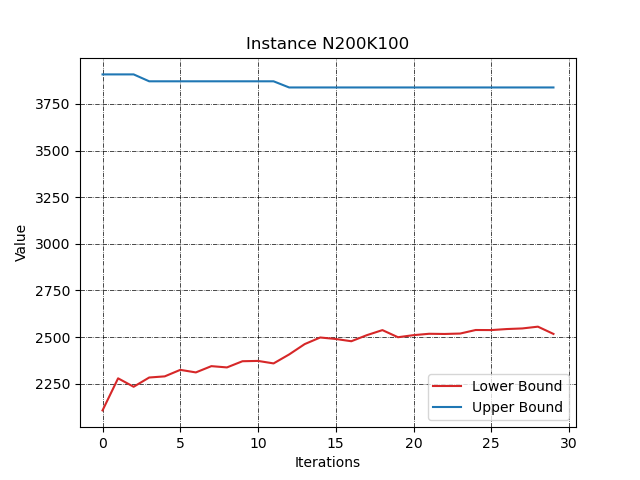
\includegraphics[width=\textwidth]{images/N200K100.png}
%     \label{fig:N200K100}
% \end{figure}

% \begin{figure}[]
%     \centering
%     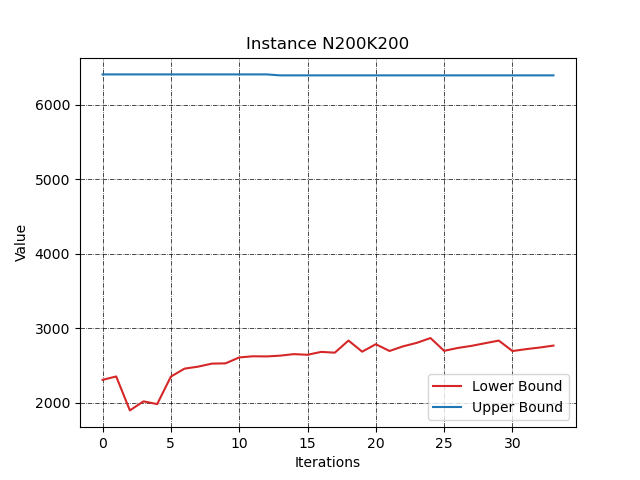
\includegraphics[width=\textwidth]{images/N200K200.png}
%     \label{fig:N200K200}
% \end{figure}

% \begin{figure}[]
%     \centering
%     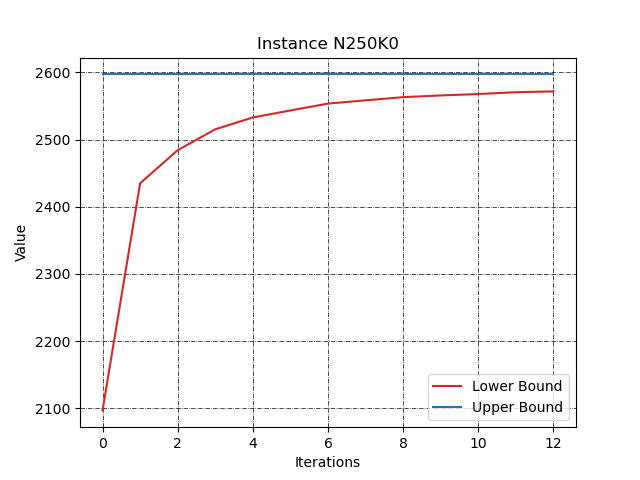
\includegraphics[width=\textwidth]{images/N250K0.png}
%     \label{fig:N250K0}
% \end{figure}

% \begin{figure}[]
%     \centering
%     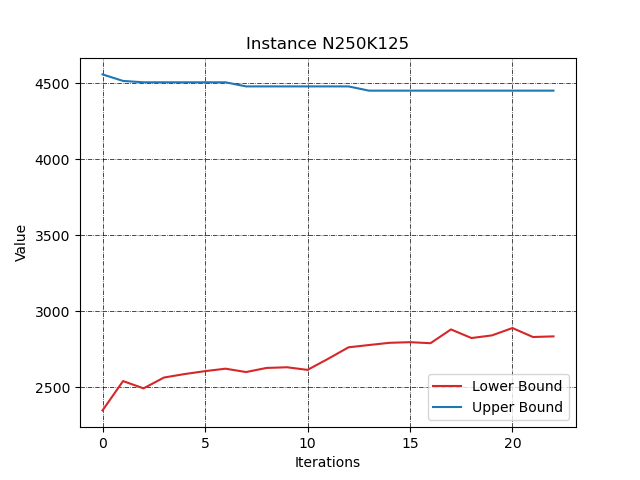
\includegraphics[width=\textwidth]{images/N250K125.png}
%     \label{fig:N250K125}
% \end{figure}

% \begin{figure}[]
%     \centering
%     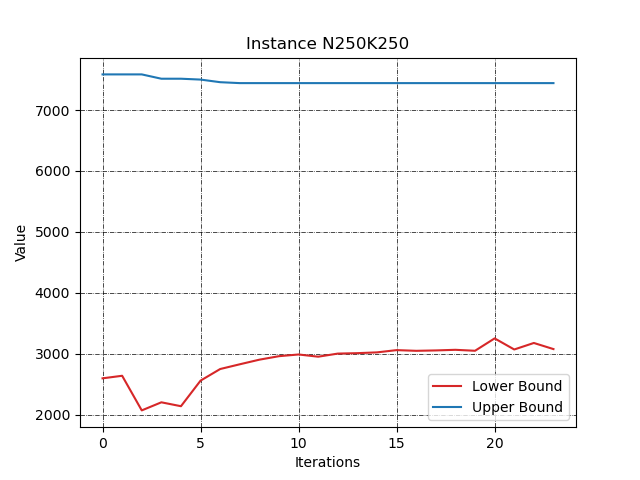
\includegraphics[width=\textwidth]{images/N250K250.png}
%     \label{fig:N250K250}
% \end{figure}

\section{Análise dos Resultados}

Nota-se que um dos passos do Algoritmo \ref{alg:kstsp} e encontrar duas soluções independentes de TSP, um para cada conjunto de distâncias fornecidas. Mas quando o fator de similaridade $\similarity$ é zero, essa é justamente a solução ótima. Portanto, para tais casos, o algoritmo encontra a solução ótima no primeiro passo. Isso significa que o Upper Bound \upperbound nunca será atualizado. Já o Lower Bound \lowerbound depende dos multiplicadores \lagrange escolhidos. A solução ótima do Dual Lagrangiano \ref{eq:goal lagrangian} é então atingida quando $\lagrange = 0$. No caso em questão, $\similarity = 0$ e portanto a solução do problema da Subseção \ref{subsec:z problem} é $\Z = 0$. Isso faz com que o subgradiente $g$ no Algoritmo \ref{algorithm:subgradient} seja sempre negativo, i.e. a solução de fato direciona-se para $\lagrange = 0$. Tudo isso pode ser visto nos gráficos de ``similaridade = 0''. Neles, o Upper Bound \upperbound é constante, enquanto que o Lower Bound \lowerbound dirige-se para a solução ótima.

Para a solução de todas as instâncias, foi dado um tempo limite de 10 minutos (600 segundos). Em muitos casos, foi tal critério que fez a execução do algoritmo parar. Em alguns casos, o tempo excedeu o limite devido a detalhes de implementação da verificação de limite de tempo. O algoritmo checa tal limite apenas no reinício do loop, de forma que sua nunca é interrompida. Isso poderia ser melhorado, mas para os objetivos da atividade não houve tal necessidade.

Nos outros casos, foi o critério de passo mínimo $\learningrate$ que definiu a parada do algoritmo. Toda vez que o Lower Bound $\lowerbound$ piora de uma iteração para a outra, o passo é reduzido. Assim, casos que apresentam bastante oscilação do Lower Bound têm maiores chances de parar por tal critério. Isso é justamente o que observamos nas instâncias de 100 vértices com similaridade \similarity igual a 50 e 100, e na instância de 150 vértices com similaridade 75.

Em todos os casos, observa-se baixa variação do Upper Bound com o número de iterações. Os casos de similaridade $\similarity = 0$ já foram discutidos acima. Para os outros casos, isso pode indicar que a heurística de factibilização da solução do Dual Lagrangiano não é capaz de gerar instâncias factíveis boas. Também pode indicar que os parâmetros utilizados no algoritmo são inadequados, muito embora sejam necessárias mais investigações e experimentações para ter alguma conclusão sobre a real causa desse comportamento.

Por fim, observa-se que é obtido um gap de otimalidade, apresentado na Tabela \ref{tab:res}. Avaliações quando à qualidade de tais gaps de otimalidade seriam interessantes de um ponto de vista prático, muito embora tal análise tenha que levar em conta também outros fatores como tempo de execução. Portanto, apesar do valor prático, está fora do escopo dessa atividade qualificar tais resultados.

\bibliographystyle{ieeetr}
\bibliography{bibliography}

\end{document}
